\documentclass{beamer}

\usetheme{GNURadio}
\usepackage{palatino}
\usepackage{color}
\usepackage{tikz}
\usepackage[utf8]{inputenc}
\usepackage{listings}

\title{Opening Beer Bottles with SDR}
\institute{Martin Braun}

\date{GNU Radio Conference 2015}

\graphicspath{{./}}
\DeclareGraphicsExtensions{.png,.pdf}

%\AtBeginSection[] {%
  %\begin{frame}
    %\frametitle{Outline}
    %\tableofcontents[currentsection]
  %\end{frame}
%}

\begin{document}

\frame{\titlepage}

\section{Introduction}

\begin{frame}
  \frametitle{Background}
  \begin{itemize}
    \item<1> PhD story\ldots
    \item<2> Actually, don't believe anything this guy says
  \end{itemize}
\end{frame}

\begin{frame}
  \frametitle{Bottle Opening \& Radio: A History}
  \begin{itemize}
    \item Before radios: Lighters
    \item<2-> The indestructible: Nokia 3510
  \end{itemize}
  \hspace{2cm}
  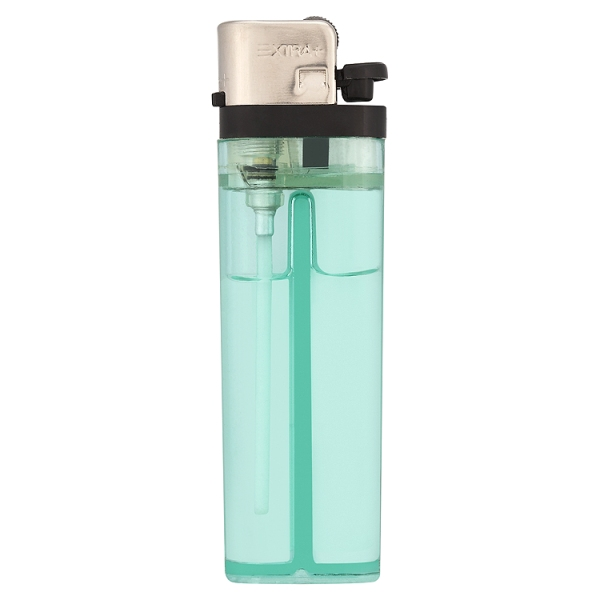
\includegraphics[height=5em]{lighter.jpeg}
  \hspace{1em}
  \includegraphics<2->[height=5em]{Nokia-3510.jpg}
\end{frame}

\begin{frame}
  \frametitle{SDR\@: The end of radio-based BBO?}
  \begin{itemize}
    \item How can we do this with software?
    \item<2-> Enter Matt Ettus, and BBO-comptible hardware
    \item<2-> USRP1, USRP2 came in solid case
    \item<2-> Most future devices worked fine as well
  \end{itemize}
\end{frame}

\begin{frame}
  \frametitle{The Physics of BBO}
  \begin{center}
  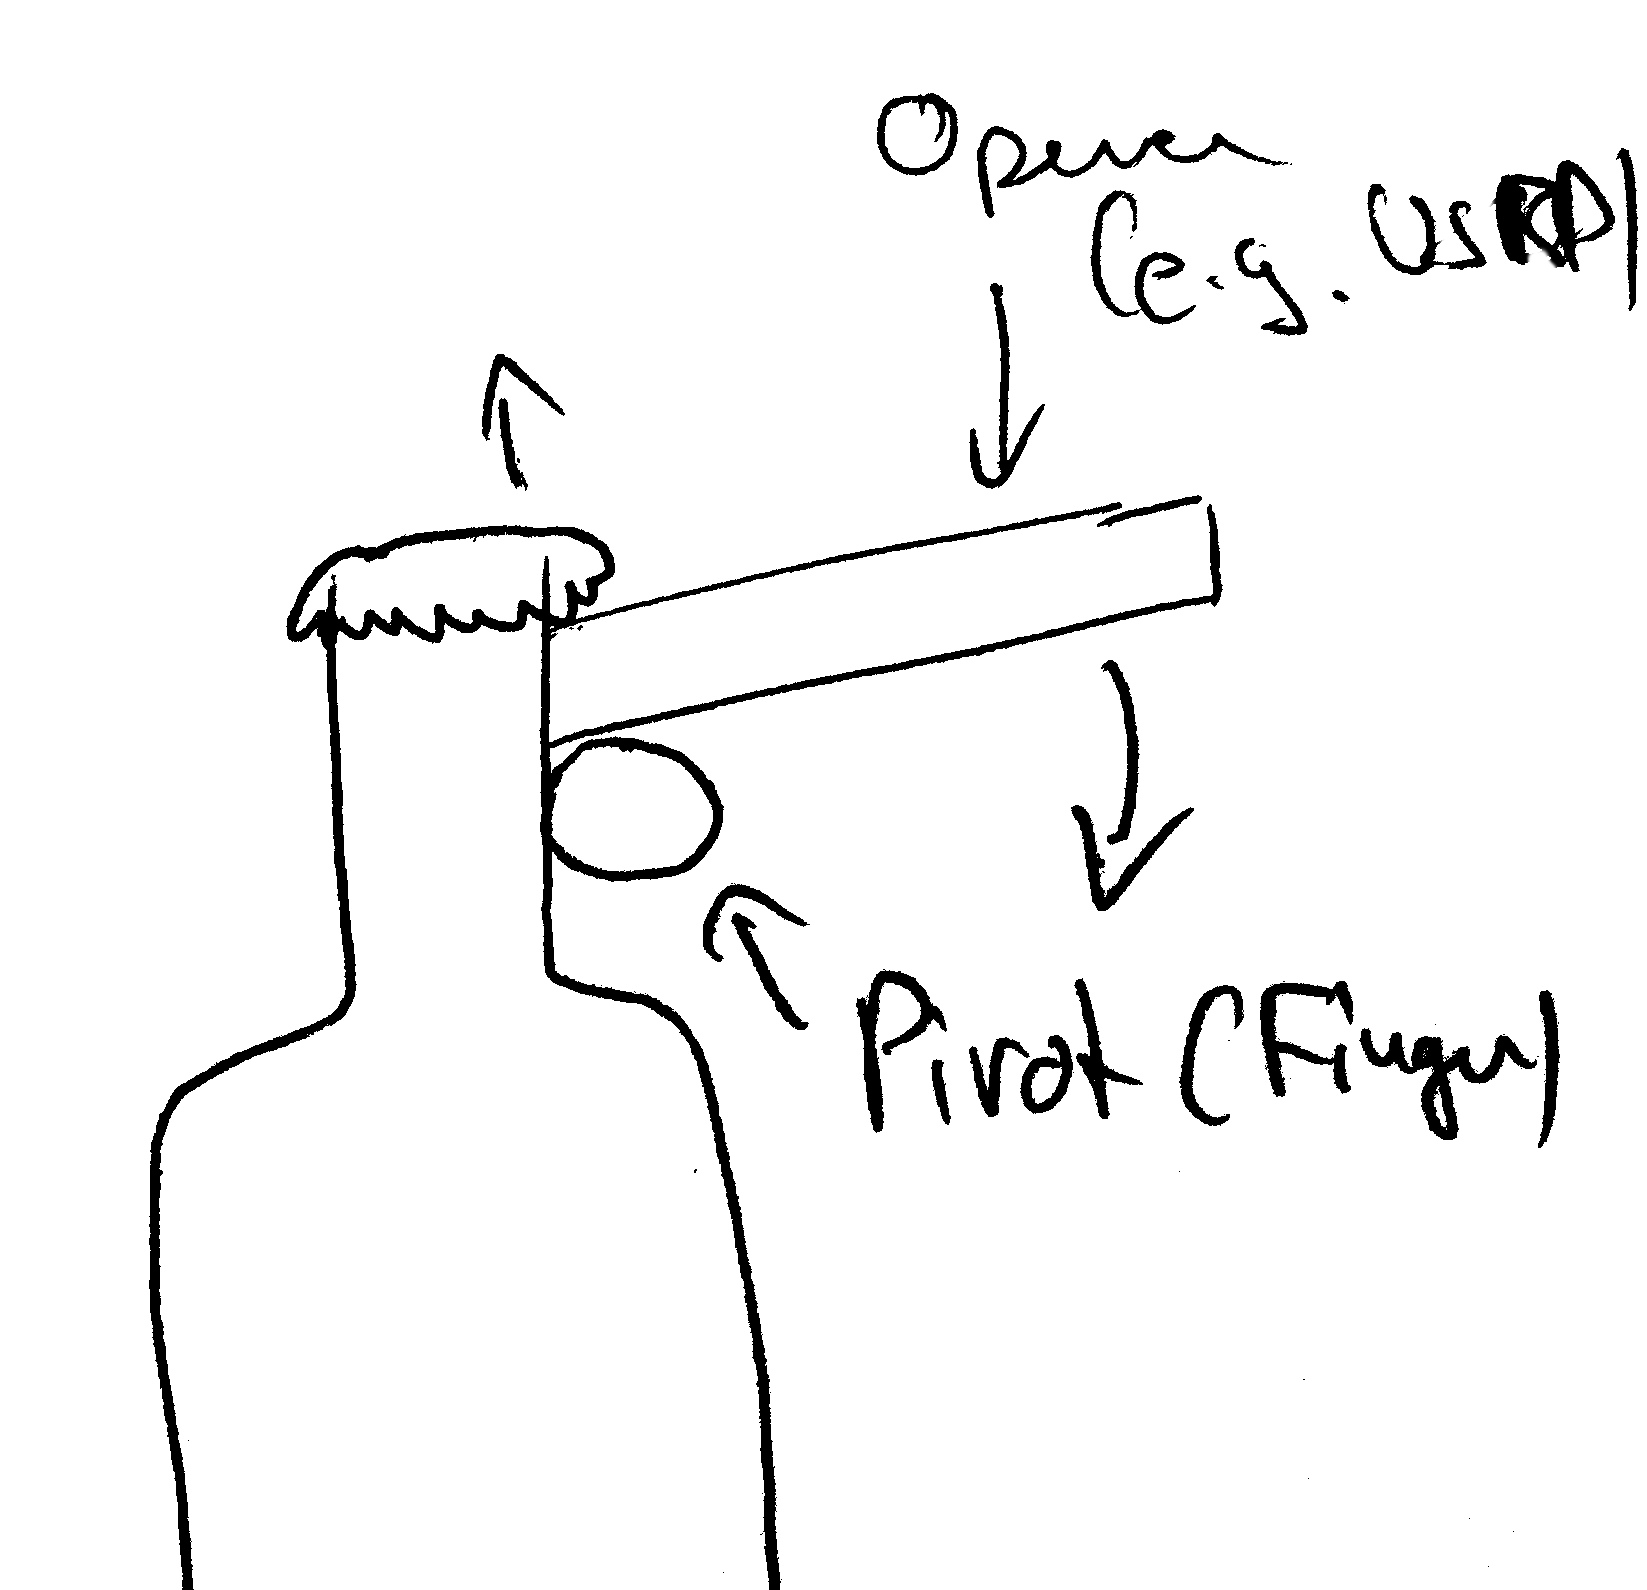
\includegraphics[height=10em]{physics.jpg}
  \end{center}
  \begin{itemize}
    \item Use: USRP, yardstick, piece of paper\ldots
  \end{itemize}
\end{frame}

\begin{frame}
  \frametitle{Random Knowledge Bombs}
  \begin{itemize}
    \item Careful with raw PCBs (in particular, baluns and other big discrete components, bending boards)
    \item Don't use USB or SMA connectors
    \item BBO'ing can scratch paint (might be a plus though)
    \item Non-alcoholic beverages may be opened, but you may be laughed at
    \item OctoClock: Use angle brackets!
  \end{itemize}
\end{frame}

\begin{frame}
  \frametitle{Summary}
  \begin{itemize}
    \item USRPs great for BBO (both professional and hobbyist)
    \item Personal favourites: E310 and B200mini
    \item Open question\@: Can we use RFNoC\@?
  \end{itemize}
\end{frame}

\end{document}
